
\chapter{Implementation Details}
In this chapter is present a description of the implementation of the project, motivating the design choices.
% In this chapter is present a description of the implementation of the project, motivating the design choices.
\section{Preliminary evaluation of the target devices}
As previously mentioned, the target of this work are the most common available recorders nowadays: smartphones. Notably, Samsung and Apple smartphones, owing to their widespread usage, have been evaluated for the project purpose. Specifically, the analysis
focused on the audio signal captured by the default recording app on each device. Additionally, an Asus Windows PC was included in the evaluation process. 
To evaluate the feasibility of the watermark, an initial analysis of the frequency response of the recording system is needed. Firstly, the analysis has been conducted by recording audio samples from the smartphone devices, inside a regular room, without a specific noise, or sound.  The power density spectrum of a not-marked recorded samples is depicted in figure\ref{fig:FR}. In all the three cases the examined file is a MPEG-4 file (.m4a extension), with a sampling frequency $Fs = 44100 Hz$, therefore the resulting hypothetical watermarking signal cannot exceed the limiting maximum frequency of about $22 kHz$.
The spectrum is extracted using Matlab's Audio Toolbox Spectrum Analyzer\footnote{The spectrum can be seen by opening Matlab "Audio Test Bench" App, setting the file reader as input, clicking the button "Spectrum Analyzer" and then running the simulation.}. 

\begin{figure}[h]
    \centering
    \begin{subfigure}{0.48\textwidth}
  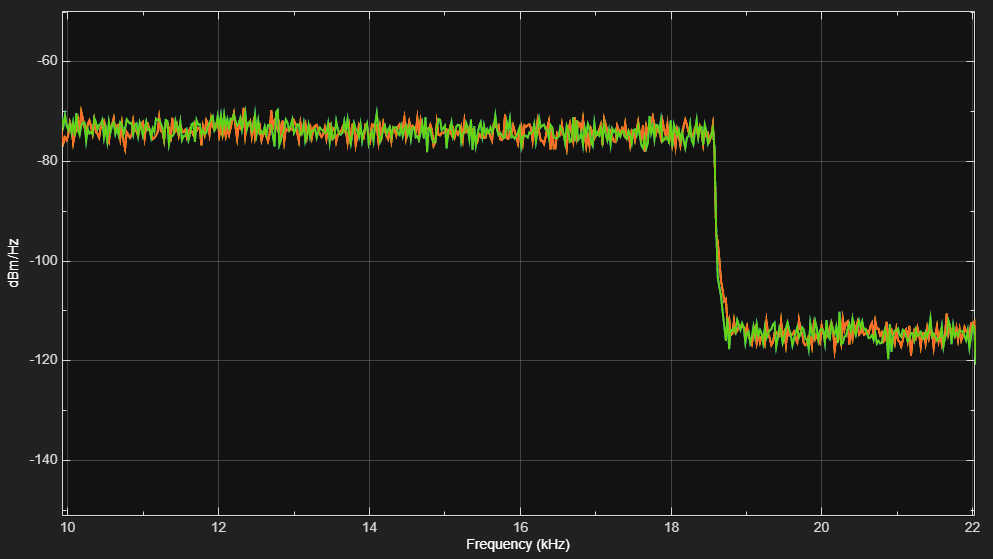
\includegraphics[width = \linewidth]{LiveAudioWatermarking/images/FRwindowsAsus.png}
    \caption{Density power spectrum of the signal recorded from Asus X507UF}
    \label{fig:FRwindows}
    \end{subfigure}
    \hfill
     \begin{subfigure}{0.48\textwidth}
      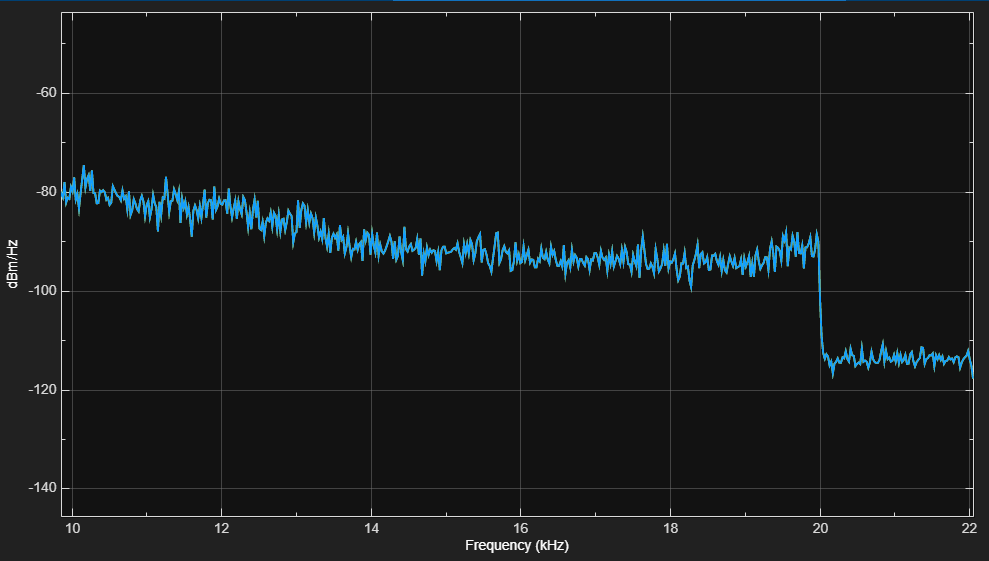
\includegraphics[width = \linewidth]{LiveAudioWatermarking/images/FRsamsung.png}
    \caption{Density power spectrum of the signal recorded from Galaxy Tab S6 Lite}
    \label{fig:FRsamsung}
    \end{subfigure}%
    \hfill
     \begin{subfigure}{0.48\textwidth}
    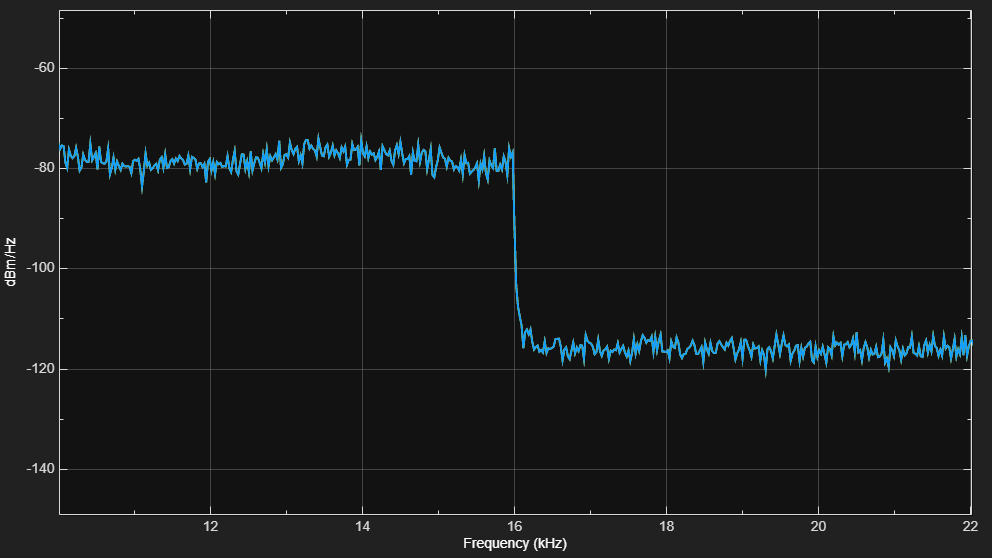
\includegraphics[width = \linewidth]{LiveAudioWatermarking/images/FRiphone14.png}
    \caption{Density power spectrum of the signal recorded from Iphone 14}
    \label{fig:FRiphone}
    \end{subfigure}%
    \caption{Frequency analysis of the signals}
    \label{fig:FR}
\end{figure}


From the results, it can be inferred that a low-pass filter is applied to the audio data, indeed the frequency response shows a the steep reduction at a certain frequency: 16kHz for iPhone, 19kHz for windows and 20kHz for Samsung. The attenuation at high frequency, in this case, may stem from both the hardware itself and the software used for recording. 
As an additional test, the response to a generated signal\footnote{The signal was generated using an \href{https://play.google.com/store/apps/details?id=com.keuwl.functiongenerator&hl=en}{Android application} on a Samsung s20+ 5G. The application's operation was validated using the computer's microphone as the input source, in "Spectrum Analyzer".} was analyzed, varying the frequency starting from 22 kHz and descending until the signal was clearly audible. The test confirmed that signals with frequency above the previously mentioned ones, are not detected, even at minimum distance and high intensity.

As a premise, it must been said that most adults have a hearing range below the 16kHz, but this value could change with respect to age (the lower the age the higher the frequency) and gender. This facts were proven by doing interviews, even though to a limited number of people. On average the best inaudibility results were obtained with frequency higher than 18 kHz, even if the generated tone remains audible to young female subjects. 

Consequently, considering watermark signal frequencies above this threshold results unfeasible with the apple products, while there is still some usable design range in Samsung's and Windows' devices.

\section{Implementation of the channel of transmission}
Considering the analysis performed by Roy et al.  \cite[page 5, BackDoor: Making Microphones Hear Inaudible Sounds]{backdoor} the solution for creating a communication channel consist in a FM modulated transmission. 
Differently from the paper approach, it is out of the scope of this project to result in a final frequency lower than the previously discussed range (e.g. 10 kHz), because it would lead to a perceivable sound in the final recording and therefore in a audible watermark. 
The channel used in this work is the data embedded in the recording with signals of which frequencies are greater or equal than 18 kHz, in order to occupy the higher end of the available spectrum.

\subsection{Evaluation of the method for transmitting data}
Digital data can be encoded and transmitted with different types of frequency modulation techniques, among the most common we selected ASK (Amplitude Shift Keying) and FSK (Frequency Shift Keying).
In FSK the frequency of the signal can assume two values: $f_{1}$ for transmitting bit '1' and $f_{0}$ for transmitting bit '0'. The binary data is therefore transmitted by means of a sine wave, which change frequency accordingly, as illustrated in figure \ref{fig:FSKbuild} 
\begin{figure}[h]
    \centering
    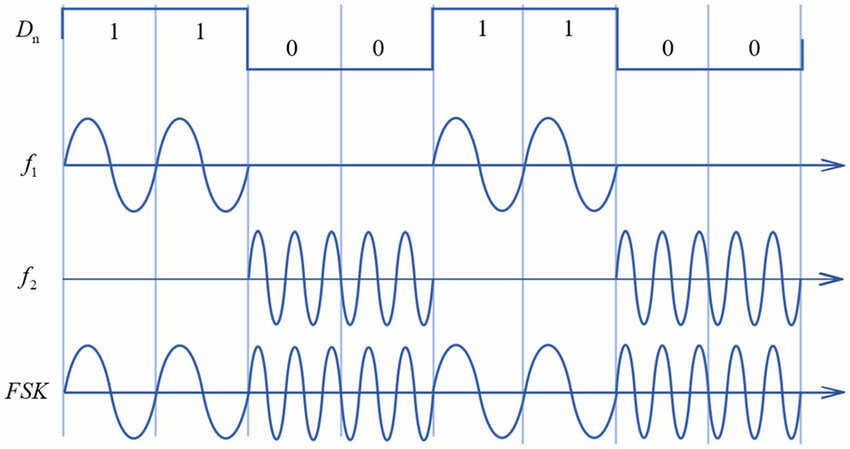
\includegraphics[width=0.8\textwidth]{LiveAudioWatermarking/images/FSK-modulation-wave-forms-example.png}
    \caption{Visual representation of the construction of an FSK modulated signal}
    \label{fig:FSKbuild}
\end{figure}

The FSK modulation can be easily transformed into a binary type of ASK, OOK (On-Off Keying), by setting one of the two frequencies at 0 Hz.
To easily detect the start and end of the transmission, two additional symbols (other than bit0 and bit1) have been added to the alphabet, therefore in a specific time interval the transmitted tone can assume 4 different frequencies ( $f_0, f_1, f_{start}$ and $ f_{stop}$). An example frame of one of the possible transmission of the character 'b' is shown in figure \ref{fig:FSK example}, from left to right represented symbols are bit start, bit0, 2 times bit1, 3 times bit0, bit1, bit0 and finally bit stop.

\begin{figure}
    \centering
    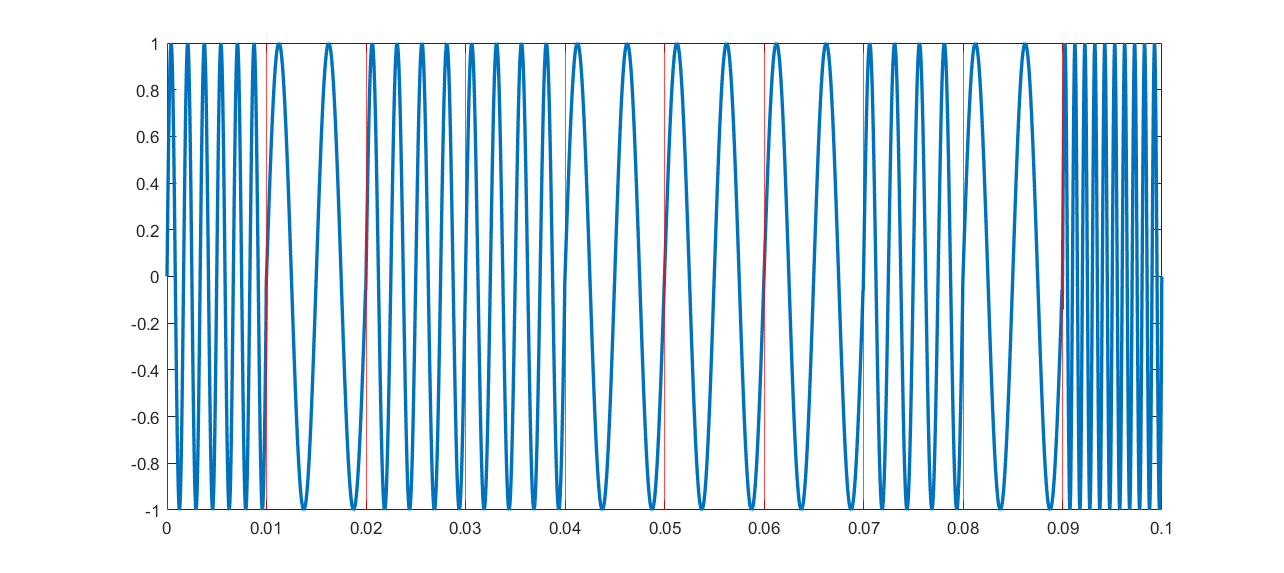
\includegraphics[width=\linewidth]{LiveAudioWatermarking/images/FSKex.png}
    \caption{Example of transmitted signal for a message composed of the character 'b'}
    \label{fig:FSK example}
\end{figure}

\subsection{Implementation of the platform used for transmitting the signal}
As previously discussed the most accessible way to use the watermark transmitter is by utilizing a smartphone app. For this purpose we developed a simple prototype application, in which the user can set the data and the parameters of the transmission. Moreover, since the application is installed on the user's smartphone, they can choose to embed meaningful information such as a real-time GPS position into the watermarking signal. The user is also able to set an encryption key that is then used to encrypt all the data to integrate in the signal through an “AES-256” algorithm, applied in Cipher Feedback Block mode, without Padding in order to keep the watermark track as short as possible. This mode can provide an additional protection against the modification of the audio sample, since, ideally, changing the order of the bits results in a message different from the transmitted one.
The application has been developed in Kotlin language, with Android Studio IDE.
The application is composed of two views: the home page and the settings.
\begin{figure}
    \centering
    \begin{subfigure}{0.30\textwidth}
        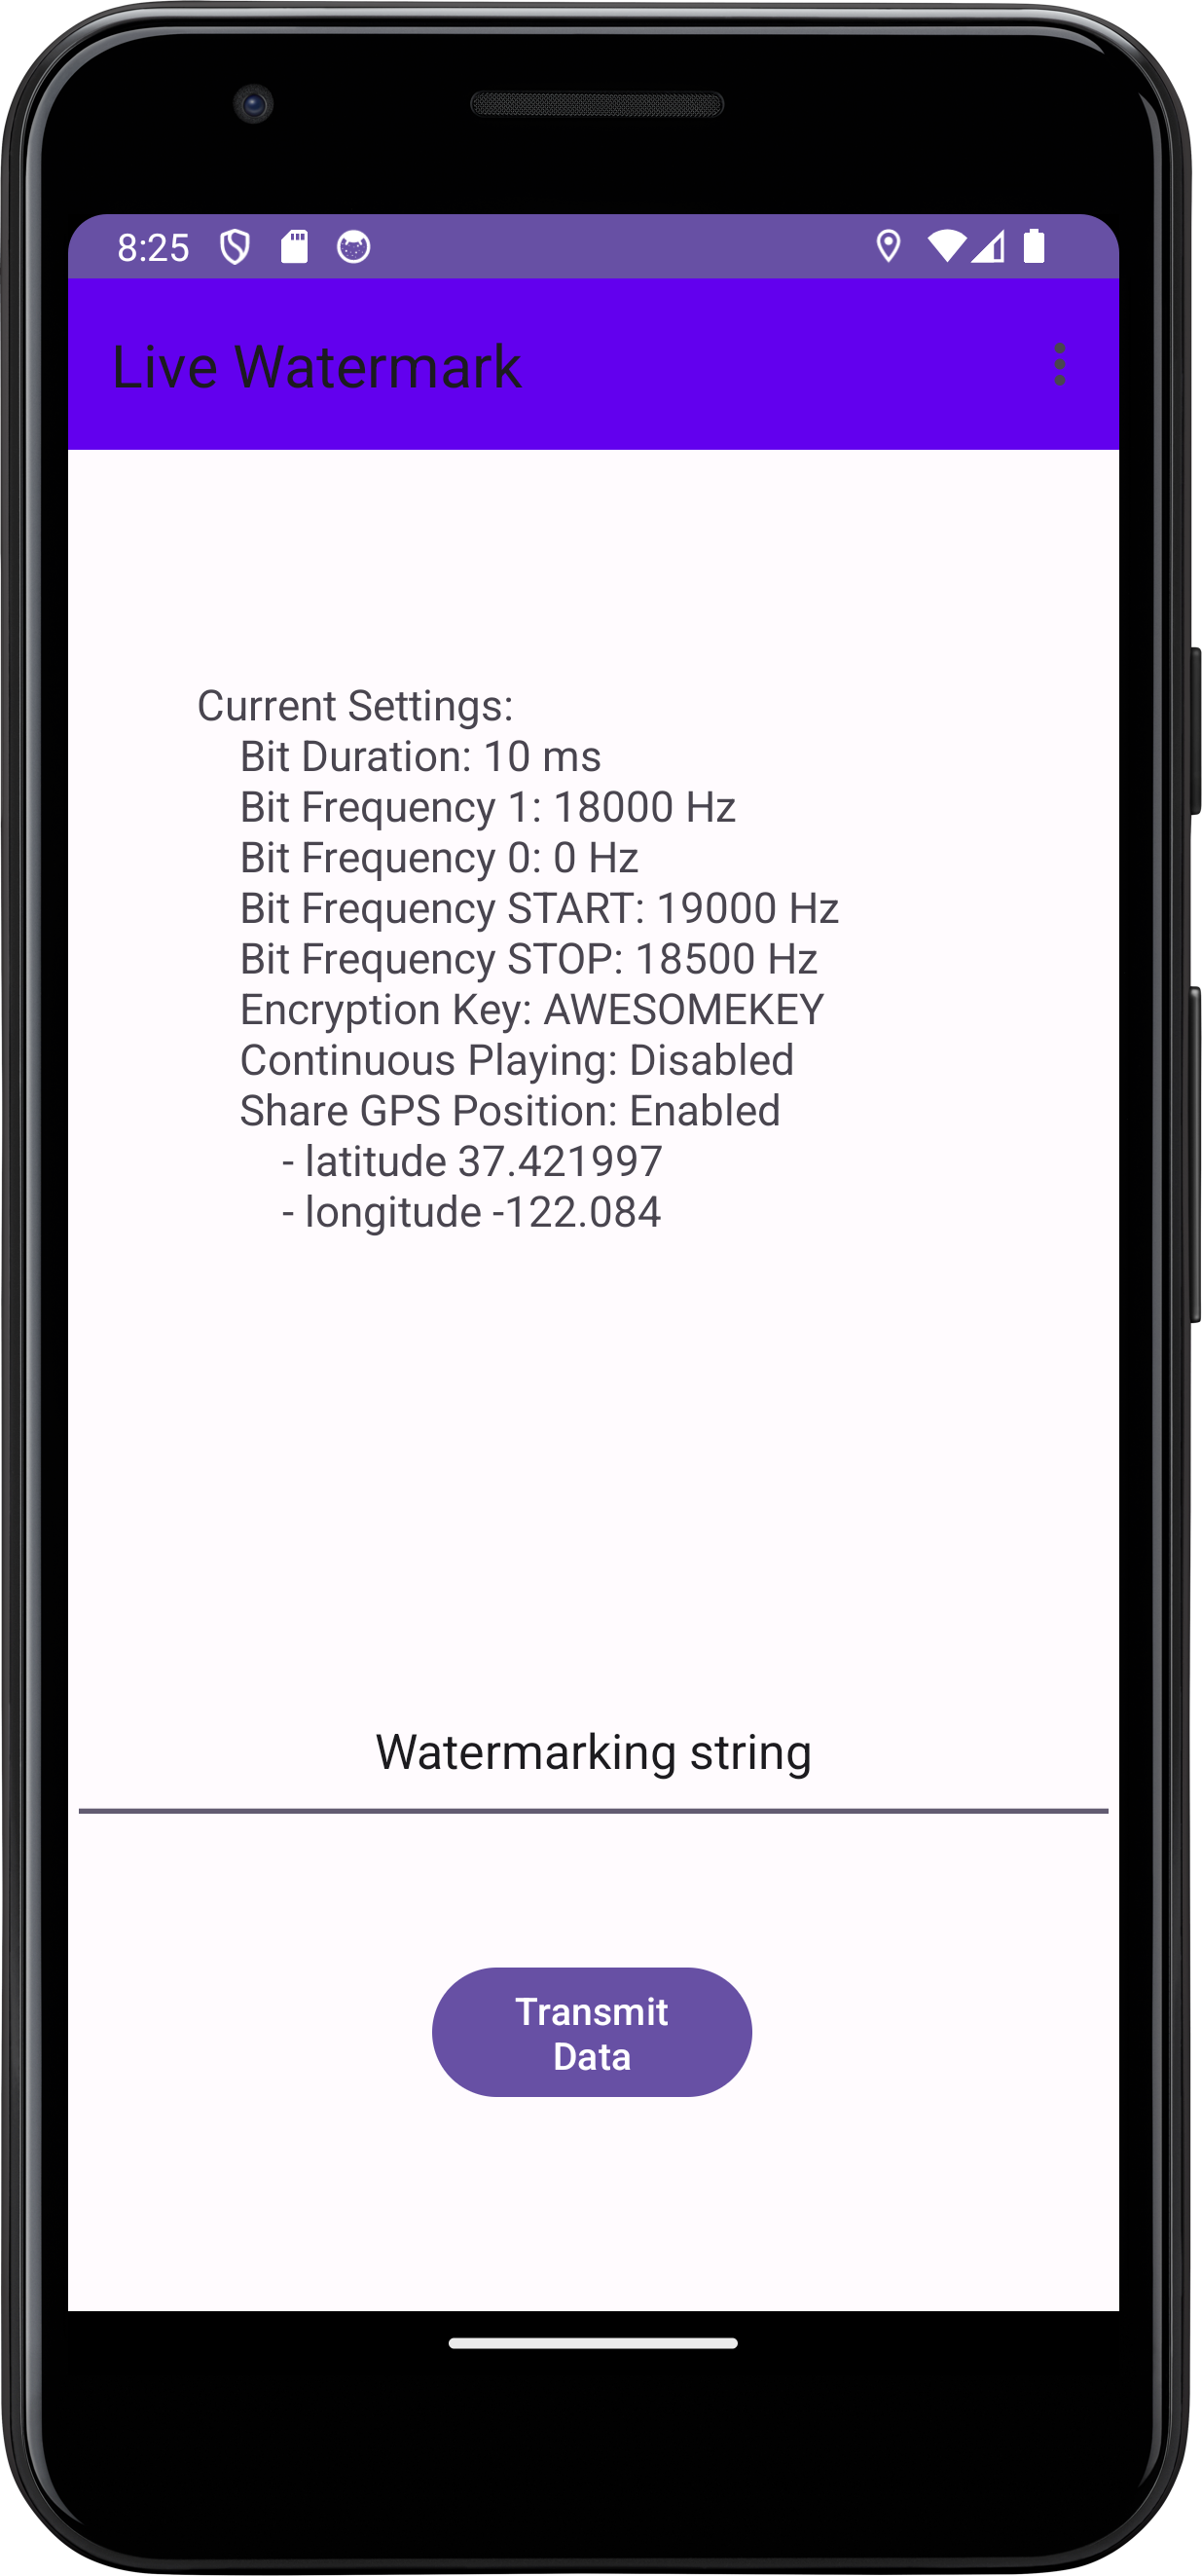
\includegraphics[width=\linewidth]{LiveAudioWatermarking/images/home_frame.png}
    \end{subfigure}
    \begin{subfigure}{0.30\textwidth}
        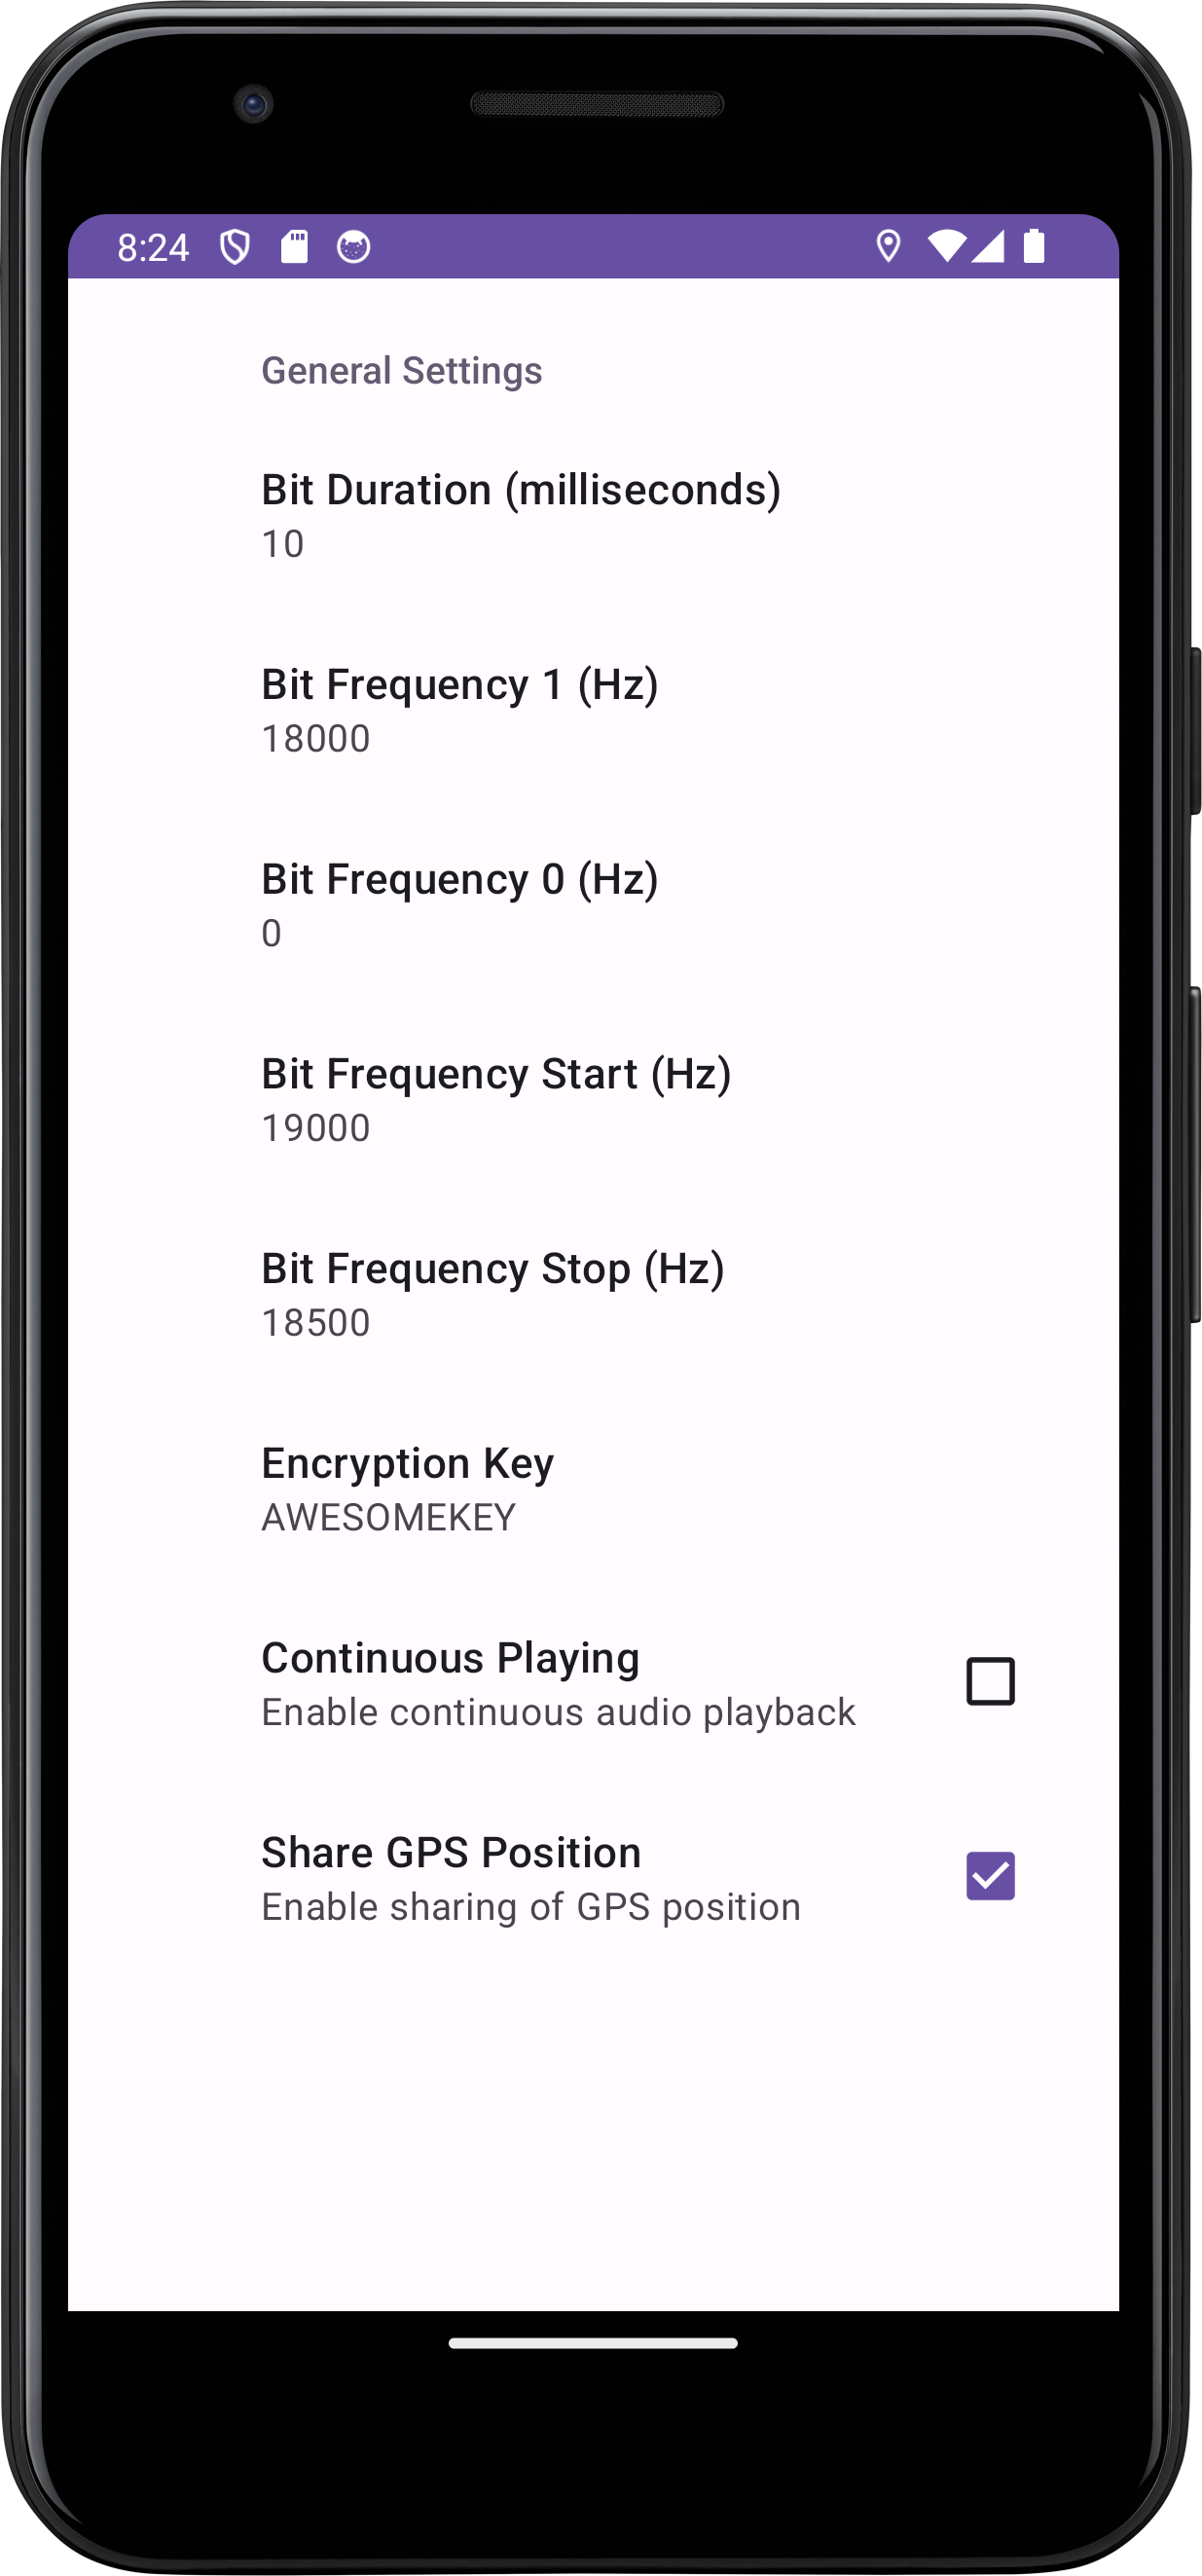
\includegraphics[width=\linewidth]{LiveAudioWatermarking/images/setting_frame.png}
    \end{subfigure}
    \caption{Main and Settings view of the application.}
    \label{fig:APP}
\end{figure}

From the main view the user can insert a string to use as a watermark. The transmission begins on pressing the "Transmit Data" button. In this prototype, there are no constraints on the format of the string or limitations on its size, except for the defaults set by the 'TextBox' object used.
In the Settings view the user can change the timing parameters previously described. The following source code shows the implementation of the transmit function, the complete code can be found in Appendix \ref{code}

\begin{lstlisting}[language=Kotlin, caption=Code of the Transmit and encrypt Function.]        
    private fun transmitData(data: ByteArray) {
        val minBuff = AudioTrack.getMinBufferSize(
            44100,
            AudioFormat.CHANNEL_OUT_MONO,
            AudioFormat.ENCODING_PCM_16BIT
        )
        val audioTrack = AudioTrack(
            AudioManager.STREAM_MUSIC,
            44100,
            AudioFormat.CHANNEL_OUT_MONO,
            AudioFormat.ENCODING_PCM_16BIT,
            max((44100 * BIT_DURATION / 1000 * data.toString().length), minBuff),
            AudioTrack.MODE_STREAM
        )
        audioTrack.play()
        val bitData = dataToBits(data)
        val start = generateTone(FREQ_BIT_START, BIT_DURATION)
        val stop = generateTone(FREQ_BIT_STOP, BIT_DURATION)
        audioTrack.write(start, 0, start.size, AudioTrack.WRITE_BLOCKING)
        for (bit in bitData) {
            val tone = if (bit == '1') generateTone(FREQ_BIT_1, BIT_DURATION)
            else generateTone(FREQ_BIT_0, BIT_DURATION)
            audioTrack.write(tone, 0, tone.size, AudioTrack.WRITE_BLOCKING)
        }
        audioTrack.write(stop, 0, start.size, AudioTrack.WRITE_BLOCKING)
        handler.postDelayed({
            audioTrack.stop()
            audioTrack.release()
        }, 100 * BIT_DURATION.toLong()) //delay added to finish the transmission before stop
    }

 private fun encrypt(plaintext: ByteArray, input_key: String): ByteArray {

        val key: SecretKey = SecretKeySpec(input_key.padStart(32, '0').toByteArray(), "aes")

        val emptyArray = byteArrayOf(
            0x00,0x00,0x00,0x00,0x00,0x00,0x00,0x00,0x00,0x00,0x00,0x00,0x00,0x00,0x00,0x00
        )

        // set cipher and options
        val cipher = Cipher.getInstance("AES/CFB/NOPADDING")
        cipher.init(Cipher.ENCRYPT_MODE, key, IvParameterSpec(emptyArray))

        return cipher.doFinal(plaintext)
    }

    \end{lstlisting}
The code makes use of other implemented function:
\begin{itemize}
    \item \texttt{dataToBits}: is a function that generates the binary string of the data
    \item  \texttt{generateTone}: is the function responsible of generating the vector containing the value of the tone to write on the stramed audioTrack.
    \item \texttt{encrypt}\footnote{Not explicitly called by the function, but conditionally executed on \textit{data} argument before it is called.}: is the function that apply the encryption algorithm. In this simple prototype, the Initialization Vector is a string of zeros. To enhance uniqueness and unpredictability, alternative approaches can be adopted, such as incorporating additional data or a combination of different data points, such as the device serial number, IMEI or a timestamp.
\end{itemize}

\section{Post-processing of the signal to retrieve the data}
To simplify the post processing identification of the data, it has been considered OOK-like transmission, with default parameters $f_{1}=18 kHz$, $f_{start}=19 kHz$, $f_{stop}=18.5 kHz$ and $tone\_length = 10 ms$. 

The analysis on the Audio track has been pursued with the help of Matlab. In particular, to automate the process and show the details of the signal, a Matlab Live Script has been coded. The script can be found in Appendix \ref{code}.

Below, the steps and methods applied to extract the embedded data from the recorded audio file are described.

\begin{enumerate}
    \item \textbf{extraction of the audio data from the MPEG-4 file}\\
    The data is stored into a vector using the program function ''audioread'', which extracts both the audio data and the sampling frequency from the file.
    \item \textbf{preliminary frequency analysis to prove the existence of the watermarking data}\\
    The analysis is made by performing the fft function on the vector of signal's data and observing the magnitude at the previously mentioned frequencies. 
    \item \textbf{Extraction of the raw watermark signal} 
    The frequencies of interest are simply isolated through a band pass filter, exploiting Matlab's \textit{bandpass} function.
    
    \item \textbf{Frequency analysis with efficient DFT algorithm}\\
    The algorithm used is Goertzel algorithm, which is very efficient for detecting the presence of a particular frequency component in a signal. It is more computationally efficient than the Fast Fourier Transform (FFT) for detecting a single frequency component. The algorithm calculates the discrete Fourier transform (DFT) of a specific frequency directly, without the need to compute the entire spectrum as FFT does. It is often used in applications such as tone detection in telecommunications and audio processing. The resulting magnitudes are used to compute the thresholds used in the next step.
    
    \item \textbf{Derivation of the transmitted binary string} \\
    The segment of the vector containing the watermark is isolated and extracted by searching the start and stop bit. To search for the right index, a cross correlation with a generated bit start tone is computed, the index of the maximum in the resulting vector represent the delay at which the start(stop) tone is found. Knowing the positions of these bits, it is possible to compute the number of tones present in the sample. Consequently each one segment is analyzed with Goertzel algorithm and compared against the threshold, which consists of the previous threshold multiplied by a constant empirically defined.
    
    \item \textbf{Decryption and interpretation of the binary string}\\
    If the transmitted data is encrypted, it can be decrypted using the provided tool, whose decrypting function code is listed here, the full code can be found in Appendix \ref{code}.
\begin{lstlisting}[language=Kotlin]
    fun decrypt(ciphertext: ByteArray, input_key: String): ByteArray {

    // exactly same code as function "encrypt" but in decryption mode
    val key: SecretKey = SecretKeySpec(input_key.padStart(32, '0').toByteArray(), "aes")
    val iv = byteArrayOf(0x00, 0x00, 0x00, 0x00, 0x00, 0x00, 0x00, 0x00, 0x00, 0x00, 0x00, 0x00, 0x00, 0x00, 0x00, 0x00)
    val cipher = Cipher.getInstance("AES/CFB/NOPADDING")
    cipher.init(Cipher.DECRYPT_MODE, key, IvParameterSpec(iv))

    return cipher.doFinal(ciphertext)
}
\end{lstlisting}
The code use the same library and approach that can be found in the application code.

\end{enumerate}


Also a variant of the live script has been developed, it simply record some second of the input data and then performs the same analysis

%retriving the sample, isolating the freq of interest, apply goertzel algorithm to analyze the energy of the signal at each frequency and calculate the thresholds, searcing for start bit  and stop bit, calculating the number of simbols, divide the signals into intervals and then evaluating again the content of the interval compared to the thresholds


% This is where you explain what you have implemented and how you have implemented it. Place here all the details that you consider important, organize the chapter in sections and subsections to explain the development and your workflow.\\Given the self-explicative title of the chapter, readers usually skip it. This is ok, because this entire chapter is simply meant to describe the details of your work so that people that are very interested (such as people who have to evaluate your work or people who have to build something more complex starting from what you did) can fully understand what you developed or implemented.\\Don't worry about placing too many details in this chapter, the only essential thing is that you keep everything tidy, without mixing too much information (so make use of sections, subsections, lists, etc.). As usual, pictures are helpful.